\documentclass[a4paper,11pt]{article}
\usepackage{setspace}
\onehalfspacing
 
\usepackage{titlesec}
\usepackage{graphicx}
\usepackage{listings}
\usepackage{xcolor}
\usepackage{fancyhdr}
\usepackage[a4paper,margin=1in]{geometry}
\usepackage{mdframed} %nice frames

\definecolor{light-gray}{gray}{0.95} %the shade of grey that stack exchange uses

\renewcommand{\thispagestyle}[1]{} % do nothing

\lstset{
  language=Python,
  aboveskip=3mm,
  belowskip=3mm,
  showstringspaces=true,
  columns=flexible,
  basicstyle={\small\ttfamily},
  numbers=none,
  numberstyle=\tiny\color{gray},
  keywordstyle=\color{blue},
  commentstyle=\color{red},
  breaklines=true,
  breakatwhitespace=true,
  tabsize=2
}

\graphicspath{ {./images/} }
\titlespacing{\section}{0pc}{1pc}{1pc}
 
\pagestyle{fancy}
\fancyhf{}
\rhead{Assignment 4}
\lhead{Design \& Implementation: Internet Video, Voice \& Text Chatting Program}
\rfoot{Page \thepage}

 
\begin{document}
\title{\vspace{-1.0cm}\textbf{Design \& Implemenation: \linebreak Internet Video, Voice \& Text Chatting Program}}
\author{
  \textbf{Tan Wei Xuan (49003140)}\\
  \texttt{tanweixuan@postech.ac.kr}
  \and
   \textbf{Zhang Xin Yue (49003143)}\\
  \texttt{xyzhang@postech.ac.kr}
}
\date{\today}
\maketitle

\section{Project Overview}
The\textbf{ Internet Video, Voice and Text Messaging Program} that I have implemented is a \textbf{Multi-threaded Chat Application} that utilises the Transmission Control Protocol \textit{(TCP)} and allows for mutiple clients to send/receive text, voice messages as well as a video stream over a server, to one another, at the same time. The source code files are as follow:
\begin{enumerate}
	\item \textbf{Server Files}
\begin{itemize}
  	\item server.py
\end{itemize}
	\item \textbf{Client Files}
\begin{itemize}
  	\item client.py
\end{itemize}
\end{enumerate}

\section{Environment and Dependencies}
My program is written in \textbf{Python 3.6.7} and is developed on \textbf{Windows running the Ubuntu 18.04.2 bit subsystem}, using \textbf{PyCharm} as the \textbf{Integrated Development Environment}. \textit{The program may not work as inteneded if it is ran on other environments.}
\textit{\textbf{Ensure that these dependencies are being installed on your system}}.
\begin{enumerate}
  \item \textbf{PyAudio}
\begin{mdframed}[backgroundcolor=light-gray, roundcorner=30pt,leftmargin=1, rightmargin=1, innerleftmargin=5, innertopmargin=-3,innerbottommargin=5, outerlinewidth=1, linecolor=light-gray]
\begin{lstlisting}
#On Ubuntu Terminal
$ sudo apt-get install python-pyaudio python3-pyaudio
\end{lstlisting}
\end{mdframed}
  \item \textbf{Threading}
\begin{mdframed}[backgroundcolor=light-gray, roundcorner=30pt,leftmargin=1, rightmargin=1, innerleftmargin=5, innertopmargin=-3,innerbottommargin=5, outerlinewidth=1, linecolor=light-gray]
\begin{lstlisting}
#On Ubuntu Terminal
$ sudo apt install python3-pip #Only if pip is not installed
$ pip install threaded
\end{lstlisting}
\end{mdframed}
  \item \textbf{libasound}
\begin{mdframed}[backgroundcolor=light-gray, roundcorner=30pt,leftmargin=1, rightmargin=1, innerleftmargin=5, innertopmargin=-3,innerbottommargin=5, outerlinewidth=1, linecolor=light-gray]
\begin{lstlisting}
#On Ubuntu Terminal
$ sudo apt-get install libasound2-devf
\end{lstlisting}
\end{mdframed}
  \item \textbf{Pillow}
\begin{mdframed}[backgroundcolor=light-gray, roundcorner=30pt,leftmargin=1, rightmargin=1, innerleftmargin=5, innertopmargin=-3,innerbottommargin=5, outerlinewidth=1, linecolor=light-gray]
\begin{lstlisting}
#On Ubuntu Terminal
$ pip install Pillow==2.2.1
\end{lstlisting}
\end{mdframed}
  \item \textbf{OpenCV}
\begin{mdframed}[backgroundcolor=light-gray, roundcorner=30pt,leftmargin=1, rightmargin=1, innerleftmargin=5, innertopmargin=-3,innerbottommargin=5, outerlinewidth=1, linecolor=light-gray]
\begin{lstlisting}
#On Ubuntu Terminal
$ pip install opencv-python
\end{lstlisting}
\end{mdframed}
\end{enumerate}

\section{Implementation - Video Chat}

\subsection{Server - Handling Video }
Below is the handler for how a server distribute the video data that is being received from one client to another. The Video port on the server is \textit{1026}. 
\begin{mdframed}[backgroundcolor=light-gray, roundcorner=30pt,leftmargin=1, rightmargin=1, innerleftmargin=5, innertopmargin=-3,innerbottommargin=5, outerlinewidth=1, linecolor=light-gray]
\begin{lstlisting}
#Server.py
def handle_client_video(client):
	"""
	Handles Video from the given socket.
 	"""
	# Receive Video
	clients_video[client] = 1
	while client in clients_video:
            ttlrec = 0
            metarec = 0
            msgArray = []
            metaArray = []

            while metarec < 8:
                chunk = client.recv(8 - metarec)
                metaArray.append(chunk)
                metarec += len(chunk)

            length = int(chunk.decode("utf8"))

            while ttlrec < length:
                chunk = client.recv(length-ttlrec)
                if chunk == '' :
                    raise RuntimeError("Socket Connection has broken")
                msgArray.append(chunk)
                ttlrec += len(chunk)

            broadcast(b''.join(metaArray + msgArray),dtype="video", sd=client)

\end{lstlisting}
\end{mdframed}

\subsection{Client - GUI}
We utilised the \textit{Tkinter module}, an inbuilt GUI implemenation of Python's library to serve as the Graphic User Interface for our program. The video stream as well as the chat window for exchanging text messages will all be displayed on the GUI.
\begin{mdframed}[backgroundcolor=light-gray, roundcorner=30pt,leftmargin=1, rightmargin=1, innerleftmargin=5, innertopmargin=-3,innerbottommargin=5, outerlinewidth=1, linecolor=light-gray]
\begin{lstlisting}
#Client.py
#TKinter Settings
top = tkinter.Tk()
top.title("Internet Voice,Video and Text Chatting Programme")

video_frame = tkinter.Frame(top)
video_frame.pack(side=tkinter.TOP)

messages_frame = tkinter.Frame(top)
messages_frame.pack(side=tkinter.TOP)

button_frame = tkinter.Frame(top)
button_frame.pack(side=tkinter.TOP)

my_msg = tkinter.StringVar()
my_msg.set("Enter your Name")

scrllBar = tkinter.Scrollbar(messages_frame)

entry_field = tkinter.Entry(button_frame, textvariable=my_msg)
entry_field.bind("<Return>", send_text)
entry_field.pack(side=tkinter.LEFT, padx = 10)

send_button = tkinter.Button(button_frame, text="Send", command = send_text)
send_button.pack(side=tkinter.LEFT, padx = 10)

msg_list = tkinter.Listbox(messages_frame, height = 15, width =50, yscrollcommand = scrllBar.set)
scrllBar.pack(side=tkinter.RIGHT, fill=tkinter.Y)
msg_list.pack(side=tkinter.TOP, fill=tkinter.BOTH)
\end{lstlisting}
\end{mdframed}

\subsection{Client - Video Capture}
We utilised the OpenCV library for the capturing of the video stream through the use of the client's webcam. The frames being captured through the webcam are treated as \textbf{Images}
\begin{mdframed}[backgroundcolor=light-gray, roundcorner=30pt,leftmargin=1, rightmargin=1, innerleftmargin=5, innertopmargin=-3,innerbottommargin=5, outerlinewidth=1, linecolor=light-gray]
\begin{lstlisting}
#Client.py
#Capture for Webcam
cap = cv2.VideoCapture(0)

#Work around in case webcam is not opened
if cap.read() == False:
	cap.open()

\end{lstlisting}
\end{mdframed}

\subsection{Client- Sending Video}
The frame (image) being captured from the webcam is subsequently (in real-time) being sent to the server through the handler below.
\begin{mdframed}[backgroundcolor=light-gray, roundcorner=30pt,leftmargin=1, rightmargin=1, innerleftmargin=5, innertopmargin=-3,innerbottommargin=5, outerlinewidth=1, linecolor=light-gray]
\begin{lstlisting}
#Server.py
#Send Video to the server
def send_video():
	global cap

	while not stop_video.is_set():
		ret_val, img = cap.read()
		img = cv2.resize(img, (360,360))

		cv2_im = cv2.cvtColor(img, cv2.COLOR_BGR2RGB)
		pil_im = Image.fromarray(cv2_im)
		b_io = io.BytesIO()
		pil_im.save(b_io,'jpeg')
		framestr = b_io.getvalue()

		ttlsent = 0
		metasent = 0
		length = len(framestr)
		lengthstr = str(length).zfill(8)

		while metasent < 8:
			sent = client_socket_video.send(lengthstr[metasent::].encode("utf8"))
			if sent == 0:
				raise RuntimeError("Socket Connection has broken")
			metasent += sent

		while ttlsent < length:
			sent = client_socket_video.send(framestr[ttlsent::])
			if sent == 0:
				raise RuntimeError("Socket Connection has broken")
			ttlsent += sent

\end{lstlisting}
\end{mdframed}

\subsection{Client - Displaying Video Stream}
The GUI of our program displays two video streams on it. One being the client's own video capture and the other being the video stream being received from the other clients on the server. This handler reads the frame (image) from the client's own webcam and displays it on the GUI.
\begin{mdframed}[backgroundcolor=light-gray, roundcorner=30pt,leftmargin=1, rightmargin=1, innerleftmargin=5, innertopmargin=-3,innerbottommargin=5, outerlinewidth=1, linecolor=light-gray]
\begin{lstlisting}
#Client.py
#Cam Capture to Screen
def show_my_video():
	global cap
	panel = None

	while not stop_video.is_set():
		ret_val, img = cap.read()

		img = cv2.resize(img, (120, 120))

		image = cv2.cvtColor(img,cv2.COLOR_BGR2RGB)
		image = Image.fromarray(image)
		image = ImageTk.PhotoImage(image)

		if panel is None:
			panel = tkinter.Label(image=image)
			panel.image = image
			panel.place(height=110,width=110,x=256,y=5)
		else:
			panel.configure(image=image)
			panel.image = image
clientSocket.close();
\end{lstlisting}
\end{mdframed}


\subsection{Client - Receving Video}
The video data that is being recevied by the client throgh the server is handled through the function below. The video data received will be displayed on the GUI.
\begin{mdframed}[backgroundcolor=light-gray, roundcorner=30pt,leftmargin=1, rightmargin=1, innerleftmargin=5, innertopmargin=-3,innerbottommargin=5, outerlinewidth=1, linecolor=light-gray]
\begin{lstlisting}
#Client.py
# For Receiving Video
def receive_video():
	global panel
	while not stop_video.is_set():
		try:
			ttlrec = 0
			metarec = 0

			msgArray = []
			metaArray = []

			while metarec < 8:
				chunk = client_socket_video.recv(8 - metarec).decode("utf8")
				if chunk == '':
					raise RuntimeError("Socket Connection has been broken")
				metaArray.append(chunk)
				metarec += len(chunk)

			lengthstr = ''.join(metaArray)
			length = int(lengthstr)

			while ttlrec < length:
				chunk = client_socket_video.recv(length - ttlrec)
				if chunk == '':
					raise RuntimeError("Socket Connection has been broken")
				msgArray.append(chunk)
				ttlrec += len(chunk)

			frame = b''.join(msgArray)
			pil_bytes = io.BytesIO(frame)
			pil_img = Image.open(pil_bytes)
			img = ImageTk.PhotoImage(pil_img)

			if panel is None:
				panel = tkinter.Label(video_frame, image =img)
				panel.image = img
				panel.pack(side=tkinter.TOP, expand = True)
			else:
				panel.configure(image = img)
				panel.image = img

		except OSError:
			break

\end{lstlisting}
\end{mdframed}

\section{Running the Program}
\textit{On the client, the input for host should be \textbf{127.0.0.1} unless a specific host has been defined.}
\subsection{Terminal}
\begin{enumerate}
  \item In the terminal, run the command \textbf{\textit{python Server.py}} to start the \textbf{server}.
  \newline
  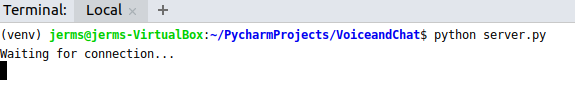
\includegraphics{server}
  \item In the terminal, run the command \textbf{\textit{python Client.py \#hostname }}to start the \textbf{client}. By default the host name will be \textbf{127.0.0.1}. The GUI will automatically be opened.
  \newline
  \includegraphics{client}
  \item Enter your \textbf{name} in the textbox and press the \textit{"Send"} button to begin using the text chat function.
  \newline
  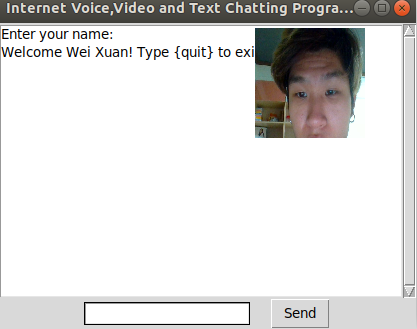
\includegraphics{name}
   \item When more than 1 user has connected to the server, both \textbf{Video} and \textbf{Voice} will be automatically enabled. You do not have to input any additional commands to enable them. \textbf{Video, Voice and Text} can be sent/received simultaneously.
   \newline
  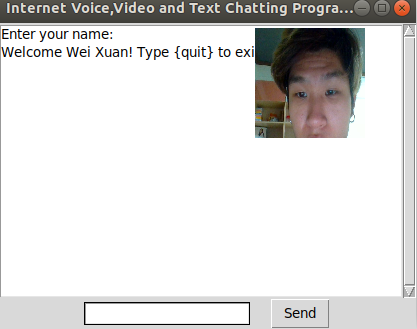
\includegraphics{name}
   \item In the \textbf{GUI Text Box}, type \textbf{\{quit\}} to exit from the server.
   \newline
\end{enumerate}

\section{Limitations}
Our Program currently only allow peer-to-peer video communications (between two parties).  Further improvement can be made to allow more than 2 clients to connect to the server and chat through video communications at any point of time. The Video Stream sent are compressed through the conversion into JPEG images and thus the resolution for then recevied Video Stream will not be of the best quality. We could implement better compression algorithms for the Video Stream to improvde the Video quality in the future.

\end{document}